\documentclass[11pt,letterpaper]{article}

% Load some basic packages that are useful to have
% and that should be part of any LaTeX installation.
%
% be able to include figures
\usepackage{graphicx}
% get nice colors
\usepackage{xcolor}

% change default font to Palatino (looks nicer!)
\usepackage[latin1]{inputenc}
\usepackage{mathpazo}
\usepackage[T1]{fontenc}
% load some useful math symbols/fonts
\usepackage{latexsym,amsfonts,amsmath,amssymb}

% comfort package to easily set margins
\usepackage[top=1in, bottom=1in, left=1in, right=1in]{geometry}

% control some spacings
%
% spacing after a paragraph
\setlength{\parskip}{.15cm}
% indentation at the top of a new paragraph
\setlength{\parindent}{0.0cm}


\begin{document}

\begin{center}
\Large
Ay190 -- Worksheet 1\\
John Pharo\\
Date: \today \\
Knights of the Realm: Anthony Alvarez, Cutter Coryell, David Vartanyan
\end{center}

\section*{Problem 1}

The purpose of the code seems to be to calculate the pressure and mass gradients of a White Dwarf. It does this by creating a grid of points representing radii from 0 to $R$, where $R$ is the radius of the surface of the star. Beginning from central values known from constants from the EOS, the code then iterates outward through the grid points, using a helper function to calculate the new pressure and mass at the new point and then checking to see if it has reached the boundary conditions of the star (eg, if the pressure has dropped below the minimum calculated for the surface, which should be essentially 0). Once the surface is reached, the code prints the total radius and mass in solar units.

\section*{Problem 2}

Using the forward Euler integrator, we get the results

\[
\begin{array}{cc}
\text{Mass (in $M_{\odot}$)} & \text{Radius (in km)} \\
1.45069351877 & 1501.5015015
\end{array}
\]

This is using the central density $\rho_c = 10^10$ g cm$^{-3}$ and a ``cut-off'' surface pressure of $P = 10^{-10} P_c$. These results agree with the problem's predictions.

\section*{Problem 3}

I was unsure whether to apply the RK steps to the pressure, and then calculate the density, or whether to just apply them directly to the density. I've tried both methods, and the error it introduces seems to be less than one percent, so as far as I can tell, it doesn't make much different which method is chosen. The results presented below are from applying the RK steps to the pressure and then calculating the density from that.

\[
\begin{array}{ccc}
\text{Method} & \text{Radius (in km)} & \text{Mass (in $M_{\odot}$)} \\
RK2 & 1537.53753754 & 1.45749016987 \\
RK3 & 1535.53553554 & 1.45742325218 \\
RK4 & 1547.54754755 & 1.45966168724
\end{array}
\]

To check the convergence rates, I use the equation for self-convergence (since
we don't know the ``true'' solution) gven in III.2.14

$$ Q_s = \frac{|y(x;h_3) - y(x;h_2)|}{|y(x;h_2) - y(x;h_1)|} $$

where $h_1 > h_2 > h_3$. I calculated $Q$ for the Forward Euler and RK2 methods by using the mass calculations at $n=1$, in order to have numbers small enough to be distinguishable. However, the calculation I get for FE is 2.0, and for RK2, approximately 3.16. These are larger than they ought to be (1 and 2, respectively). I'm not sure why this is.

\section*{Problem 4}

\begin{figure}[!htb]\centering
  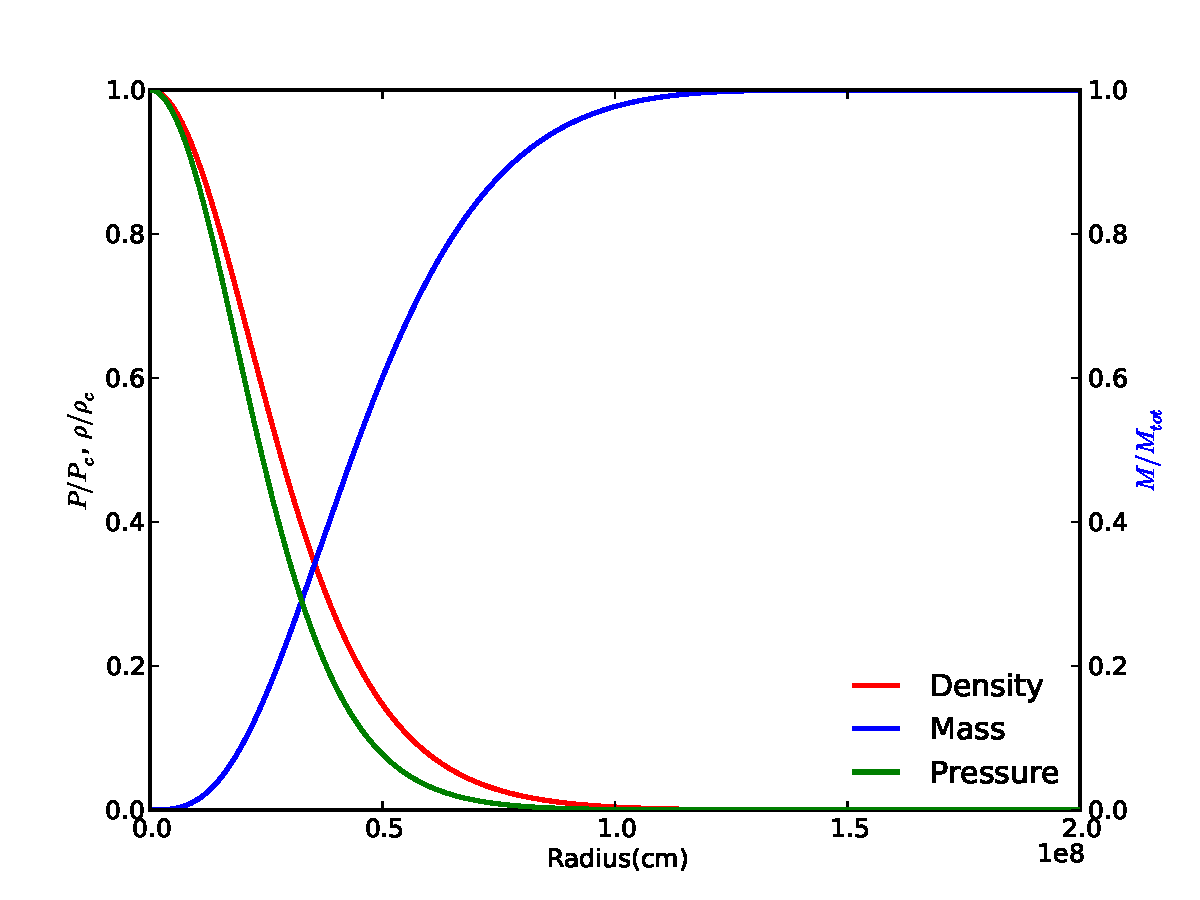
\includegraphics[width=1\textwidth]{WhiteDwarf}
  \caption{A plot of the density, pressure, and mass of the white dwarf (scaled by their maximum values) as a function of radius.}
  \end{figure}

\end{document}
